%%%%%%%%%%%%%%%%%%%%%%%%%% author.tex %%%%%%%%%%%%%%%%%%%%%%%%%
%
% sample root file for your contribution to a "contributed book"
%
% "contributed book"
%
% Use this file as a template for your own input.
%
%%%%%%%%%%%%%%%%%%%%%%%% Springer-Verlag %%%%%%%%%%%%%%%%%%%%%%%%%%


% RECOMMENDED %%%%%%%%%%%%%%%%%%%%%%%%%%%%%%%%%%%%%%%%%%%%%%%%%%%
\documentclass[12pt]{article}
\usepackage{a4wide}
\usepackage{graphics}
\usepackage{epsfig}
\usepackage{listings}
\usepackage[english]{babel}
\usepackage[latin1]{inputenc}
\usepackage{amsmath}
\usepackage{amssymb}
\usepackage{amsfonts}
\usepackage{tabularx}
\usepackage{url}
\usepackage{fancyvrb}

\usepackage{graphicx}
\usepackage{epsfig}
\usepackage{psfrag}
\usepackage{subfigure}
\usepackage{pstricks}
\usepackage{comment}


\title{Software correlation.}
\author{Nico Kruithof
\footnote{Joint Institute for VLBI in Europe (JIVE),
%  Postbus 2, 7990 AA Dwingeloo, The Netherlands
  \texttt{Kruithof@jive.nl}}
, Damien Marchal\footnote{University of Amsterdam (UvA),
%  Kruislaan 403, 1098 SJ Amsterdam, The Netherlands
  \texttt{DMarchal@science.uva.nl}
}
}
\date{}


\begin{document}

\maketitle

\abstract{Very Long Baseline Interferometry (VLBI) is a technique in
  astronomy where several distant radio telescopes observe the same
  source and the received signals are recorded and later correlated to
  produce an image with a large resolution. 

  The primary task of JIVE is the correlation of data from the EVN
  telescopes \cite{EVN} all around Europe. A special-purpose built
  hardware correlator processes the experiments. We are currently
  investigating the capabilities of a next generation software
  correlator using Grid processing power. In this paper we describe
  the design of this software correlator and some experimental
  results.}
%

\section{Introduction}
Very Long Baseline Interferometry (VLBI) \cite{VLBIbook} is a type of
interferometry used in radio astronomy, in which data received at
several telescopes is combined to produce an image with very high
resolution. VLBI can be used for both astronomy and geodesy.  For
astronomy, VLBI provides high-resolution images of radio sources in
the sky, whereas in geodesy VLBI measures the location of the
telescopes and the Earth Orientation Parameters (EOP).

Astronomical research aims to study the sky and requires high angular
resolution. The resolution of the image increases linearly with the
size of the telescope dish. However, it is not possible to build
telescope dishes of arbitrary large size.  Instead, measurements of
several telescopes can be combined using VLBI to simulate a telescope
as large as the Earth. 
%By measuring the cross correlation of the signals between all
%telescope pairs, one is able to measure the angular Fourier components
%of the image in the sky.

\subsection{VLBI}
In order to approximate a telescope with a larger dish, multiple
telescopes can observe the same object, and the data can be combined
using interferometry. A pair of telescopes forms a baseline. The
maximal frequency is defined by the two telescopes farthest apart. Due
to the rotation of the earth, these projected distances change during
an experiment giving the possibility to measure a range of spatial
frequencies with a limited number of telescopes. The angular
resolution of the VLBI array depends on the maximum projected baseline
length, while the sensitivity depends on the number of telescopes and
the bandwidth. Because the radio emission has a broad white noise
spectrum it is most efficient to use two bit (4 level) sampling of the
signal. However the data rate is a limiting factor for the total
bandwidth, as Nyquist sampling is required.

In practice, the data is recorded at the telescopes on disk packs
during a VLBI experiment. After the experiment the disks are shipped
to a central institute, e.g. the Joint Institute for VLBI in Europe
(JIVE), for correlation. At JIVE, the data from the different
telescopes is played back and correlated by a dedicated hardware
correlator~\cite{EVNCorrelator}. The maximal capacity of this hardware
correlator is 16 telescopes at a data rate of 1Gbs each. There can be
several weeks between the experiment and the time when the correlated
data becomes available.

%\marginpar{NGHK: Check 16Mb/s in table}
\begin{table}
  \centering
  \begin{tabular}[c]{|l|l|l|l|l|l|}
    \hline
    Description & \# & \#  & data-rate & spect/prod & Tflops\\
    & telescopes & sub-bands & (Mb/s) &  & \\
    \hline
    \hline
    Fabric-demo &4 &2 &16 &32 &0.16\\
    1 Gb/s, full array  &16 &16 &1024 &16 &83.39\\
    future VLBI &32 &32 &4096 &256 &\verb|~|21457\\
    \hline
  \end{tabular}
  \caption{Network bandwidths and computing power needed for an {\it e}-VLBI
    experiment based on a XF architecture.}
  \label{tab:speed}
\end{table}
\subsection{{\it e}-VLBI}
In an electronic VLBI ({\it e}-VLBI) experiment \cite{szomoru-2004},
data from the telescopes is transferred directly over the internet to
JIVE, where it is streamed into the correlator in real time. The data
transport from the telescopes to JIVE goes over several networks like
local connections, paths provided by NRENs and the G\'EANT backbone in
Europe.

The sensitivity achievable using interferometry is proportional to the
square-root of the data rate and the number of telescopes, whereas the
angular resolution is proportional to the maximal distance between two
antennas. Hence, heavy requirements are put both on the network
connections and the computing power to achieve a good sensitivity, see
also Table~\ref{tab:speed}.

Transporting the data over the network has several advantages over a
traditional experiment. Obviously, the results of the experiments are
almost immediately available. This opens up the possibility to change
the course of an experiment based on earlier findings. Also, {\it
  e}-VLBI allows for real time analysis of the data and helps to
identify and resolve minor technical problems in the data collection
during the experiment.

Several experiments in the past have shown that real time {\it e}-VLBI
is possible. The EC funds the EXPReS project\footnote{EXPReS is made
  possible through the support of the European Commission (DG-INFSO),
  Sixth Framework Programme, Contract \#026642.}~\cite{EXPReS} which
aims at building a production-level {\it e}-VLBI instrument of upto 16
intercontinental telescopes connected in real-time to JIVE and
available to the general astronomy community.

\begin{figure}
  \centering
  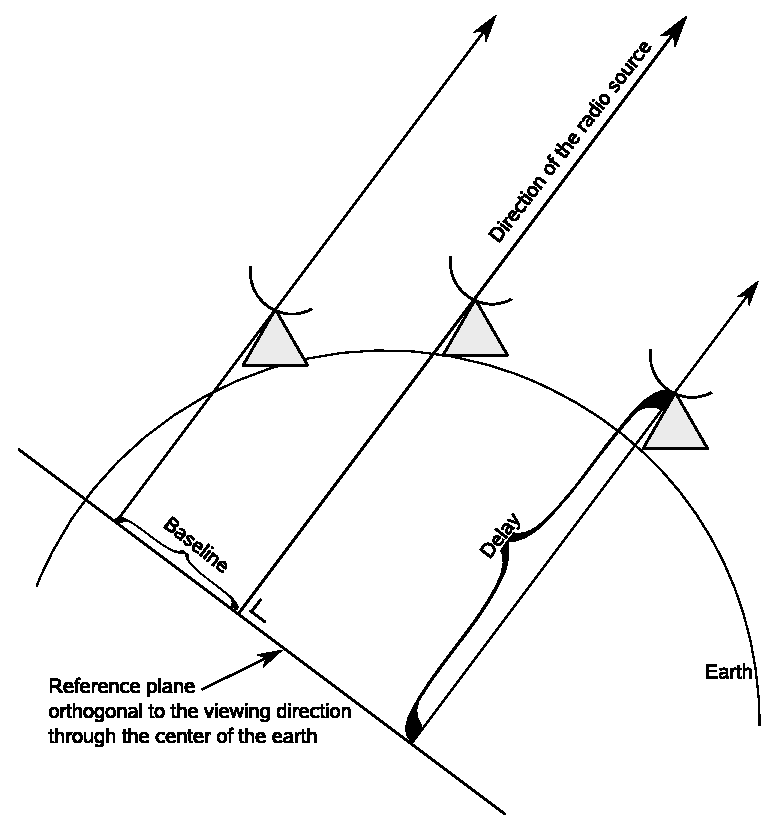
\includegraphics[width=.425\textwidth]
    {img/VLBI}
    \caption{Block diagram of the correlation.}
  \label{fig:correlation_diagram}
\end{figure}
\subsection{Correlation}
Correlation is the process by which data from multiple telescopes is
collected and combined to measure the spatial Fourier components of
the image of the sky. The high data rates and the optimizations
complicate the process.

Assume that we are correlating the signal of two telescopes. First,
both signals are delayed to account for the different time at which
the signal arrives at the telescopes, see
Figure~\ref{fig:correlation_diagram}. Next, a phase shift is performed
to compensate for the Doppler effect produced by the rotation of the
earth. This process requires very accurate timing information in the
data and a very detailed model of the geometry of the experiment. The
signals are now ready to be correlated.

During correlation, the first signal is delayed with discrete steps
and each delayed signal is multiplied with the second signal and then
integrated.  The output is a summation per delay step.

For more than two stations, each station is correlated with itself
(auto-correlation) and every other station (cross-correlation). Note
that the complexity is quadratic in the number of telescopes.

\section{Software correlator}
If the data in an {\it e}-VLBI experiment can be streamed over the internet
to JIVE, it can also be sent to another correlator. We are currently
investigating the possibilities of a next generation correlator using
a computing Grid. The advantages of a software correlator over a new
dedicated hardware correlator lie in its flexibility and accuracy. The
software correlator can be tuned for special experiments. The main
advantage of a dedicated hardware correlator is the greater
performance. The advance of general purpose computing is making
software correlation a cost-effective solution for a range of
applications. A similar approach is presented in \cite{deller-2007}.

The flexibility of its design allows the software correlator to change
with the needs of researchers. In fact, the first version of the
software correlator was developed to track the Huygens spacecraft
during its descent through the atmosphere of Saturn's moon Titan. Due
to the nature of this experiment, special requirements are put
on the correlator, which the current hardware correlator is not able
to provide.  Moreover, we expect that the costs of developing a
software correlator are much lower than the costs for a hardware
correlator.

The correlation is done by splitting the signal in time slices that
are processed in parallel (see Figure~\ref{fig:netw_corr}). The signal
from a telescope is received by a single so-called data node.  The
data node sends slices of data to an available correlate node. The
correlate node receives data from all telescopes for a certain time
slice and performs the correlation. The size of the output of the
correlation is much smaller than the input size and can be collected
and stored by a single output node.  There is one manager node that
assigns data to available computing nodes.

The correlation is not computationally expensive, in the sense that it
requires only few operations per transferred bytes. However, due to
the high data rates, the absolute number of clock cycles required by
the application is still extremely high. Moreover, the problem is
quadratic in the number of telescopes participating in the experiment
since it is linear in the number of channel pairs that have to be
correlated. The huge need for networking and computing power makes a
computing Grid an ideal platform for this application.


\begin{figure}
  \centering
  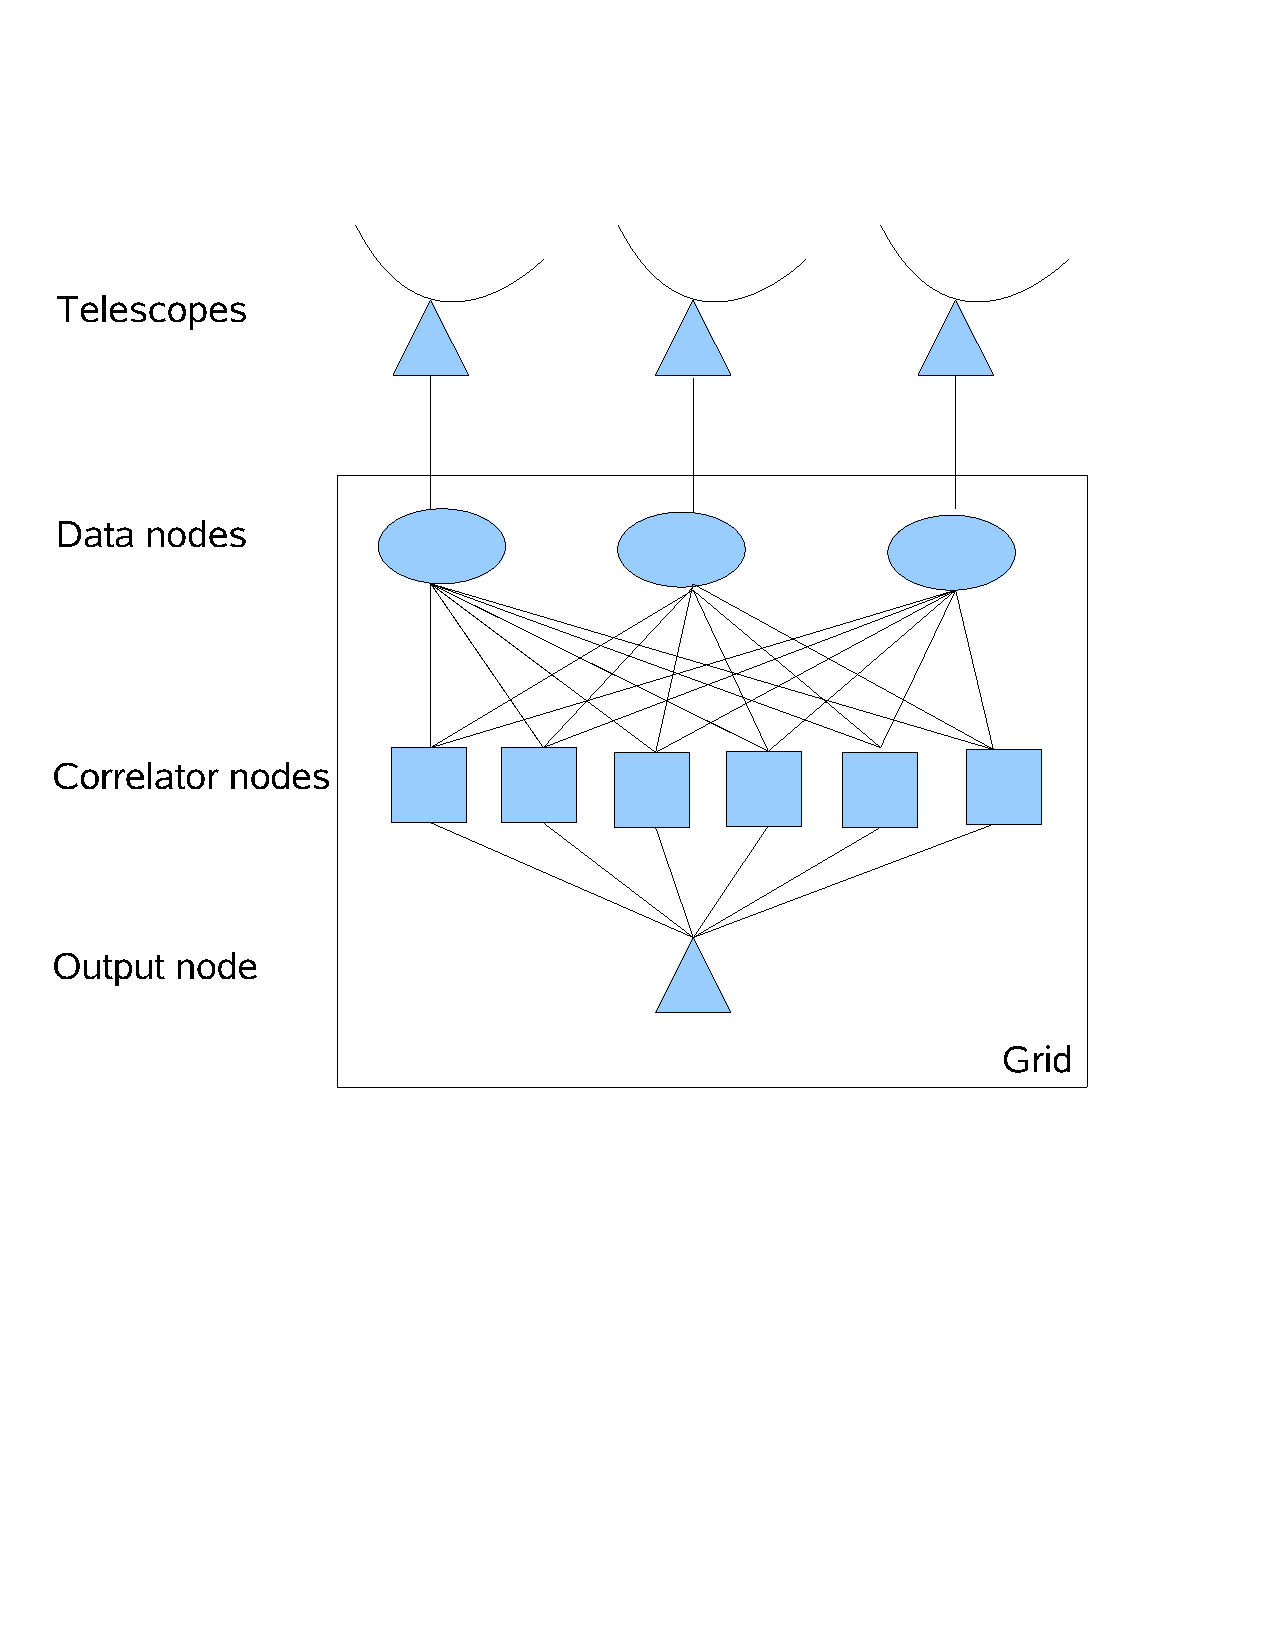
\includegraphics[width=.45\textwidth]
    {img/NetworkConnections}
    \caption{Outline of the network connections between different
      components in the software correlator.}
  \label{fig:netw_corr}
\end{figure}


\subsection{Design}
The software correlator is written in \verb~C++~ and uses several
standard libraries like \verb~fftw~ \cite{FFTW05}, \verb~mpich~
\cite{Gropp:1996:HPI} and the standard template library.

At initialization, each node is assigned a role: data node, correlator
node, output node or manager node. The node then creates a number of
controllers that manage different tasks of the node. For example there
are controllers for reading input, processing the data and writing the
output. A single type of controller can be used by different kinds of
nodes. If a node receives a message, it delegates the message to the
different controllers. The proper controller can then process the
message.

\paragraph{Data node}
The data node opens a controller for reading data and a controller for
forwarding the data to the correlate nodes. It then connects the two
using a buffer. The data node will receive a message from the manager
node specifying how to obtain the input: from file or over the network
using one of various types of transfer protocols. It will also receive
messages containing a start and stop time and the correlate node to
send the data to.

\paragraph{Correlate node}
A correlate node will initialize the correlation process and connect
to the output node. It can receive messages from a data node asking to
open an input connection and from the manager node to process a
time slice. After the slice is processed the node will send a message
to the manager node saying it is available for a next job.

\paragraph{Output node}
The output node will receive a message from the manager node where
to store the data, and it allows connections from the correlate node to
be opened. The node sorts the received data from the correlate nodes
and stores it for further processing. The output node has to make the
received data available to the user, and it should be archived in a
proper way.

\paragraph{Manager node}
The manager node is the most complicated node in the software
correlator. It sends messages to initialize the other nodes and tells
them how to connect to each other. After the initialization, it
maintains a list of available correlate nodes and delegates time
slices to available correlate nodes. General error messages can also
be sent from any node to the manager node.

The interface to the user will communicate with the manager node to
send commands to the correlator and obtain status information from the
correlator. The user interface will be based on Virtual lab.

\subsection{Network connections}
Since correlation is mainly a networking problem, testing and
optimizing the data flows is of vital importance for the performance
of the software correlator. We distinguish two types of data flows:
containing control messages and the signals from the telescopes. 

\paragraph{Control messages}
The control messages are sent between different nodes to regulate the
correlation. They form a low bandwidth stream and MPI is used to send
these messages. The network is mainly star shaped around the control
node, but there are some connections during the initialization between
input nodes and the correlate nodes and between correlate nodes and
the output node. Since the messages control the correlator, the
delivery of the messages has to be guaranteed.
\paragraph{Signal of the telescopes}
The signal from the telescopes requires far more bandwidth than the
control messages. The constant throughput for these connections is
very important as we are dealing with real time data. Some packet loss
is even acceptable if a data stream at a constant rate can then be
maintained. The connections for these data streams are set up to be
exchangeable such that it is possible to test different network
protocols like TCP (using jumbo frames), or protocols used for
streaming media. The network consists of three layers: from the
telescopes to the data nodes, then to the correlate nodes and finally
to the output node, as is shown in Figure~\ref{fig:netw_corr}.


\section{Future work}
Within Future Arrays of Broadband Radio-telescopes on Internet
Computing (FABRIC), which is a joint research activity in the EXPReS
project, we are currently implementing the software correlator. The
work flow management is designed by the the Polish Supercomputing and
Networking Center in Poznan.

In order to be able to guarantee data transfer, it might be necessary
to add an extra node near the telescopes with guaranteed bandwidth to
the telescope. This node could buffer the input data in case the
transfer rates to the Grid drop temporarily. When the software
correlator is run on a cluster of super computers, this node can also
send large time slices directly to alternating super computers. In
this way the network connectivity is optimized by introducing an
additional layer of input nodes.

Other research areas that need attention are found in resource
leveling, dealing with delays in data transfers and managing
insufficient computing power.

We also want to test several networking protocols to optimize the data
transfer. For example, we could imagine using UDP for the main data
stream, where some data loss is acceptable and a TCP connection for
data-headers to guarantee their proper delivery.
%
%
% BibTeX users please use
\bibliographystyle{plain}
\bibliography{biblio}
%
% Non-BibTeX users please follow the syntax
% the syntax of "referenc.tex" for your own citations
%\input{referenc}
%%%%%%%%%%%%%%%%%%%%%%%%%%%%%%%%%%%%%%%%%%%%%%%%%%%%%%%%%%%%%%%%%%%%%%

%%%%%%%%%%%%%%%%%%%%%%%%%%%%%%%%%%%%%%%%%%%%%%%%%%%%%%%%%%%%%%%%%%%%%%

\end{document}





